\date{}
\title{}
\date{}
\begin{document}
\begin{frame}
    \titlepage
\end{frame}

\begin{frame}
\frametitle{last time}
    \begin{itemize}
    \item ad-hoc and infrastructure mode
        \begin{itemize}
        \item association with SSID
        \item multiple APs per SSID
        \item distribution networks
        \end{itemize}
    \item mesh networks
    \item mobility via proxying
    \item base stations planning channel use
        \begin{itemize}
        \item broadcast periodic schedules of frequency use
        \item fallback to wifi-like ideas for `new' devices
        \end{itemize}
    \end{itemize}
\end{frame}

\section{firewall use cases}
\section{stateless firewall idea}
\begin{frame}{firewall rules}
    \begin{itemize}
    \item simple idea: look at packet's fields
    \item table indicating whether to reject
    \vspace{.5cm}
    \item similar idea to routing, but\ldots
    \item table matches fields other than destination
    \item table acitons are `drop', `reject', etc.
    \end{itemize}
\end{frame}


\begin{frame}{``stateless'' firewall}
    \begin{itemize}
    \item this design: table is set once by sysadmin
    \item doesn't change based on connections, etc.
        \begin{itemize}
        \item might change based on manual reconfiguration, etc.
        \end{itemize}
    \vspace{.5cm}
    \item called ``stateless''
    \vspace{.5cm}
    \item firewall doesn't track `state' based on current activity
    \end{itemize}
\end{frame}

\begin{frame}{exercise: what info do we need}
    \begin{itemize}
    \item what fields do we need to match these
        \begin{itemize}
        \item (and/or can we not handle without something more stateful?)
        \end{itemize}
    \vspace{.5cm}
    \item DNS queries to recursive DNS server from external servers
    \item packets with source address that does not match network
    \item from known malicious sources
    \item connecting from outside  to TCP servers not on allowlist
    \item connecting from inside using services (HTTP, etc.) not on allowlist
    \end{itemize}
\end{frame}


\subsection{nftables rules}
\begin{frame}[fragile]{Linux firewall: nftables}
\begin{itemize}
\item one version of packet filtering: Linux's nftables
\item different ``hooks'' where filtering can happen, list for IP:
    \begin{itemize}
    \item prerouting
    \item input (if received locally), forward (otherwise)
    \item output (if sent from local program)
    \item postrouting
    \end{itemize}
\item each hook has multiple ``chains'' of ``rules''
\end{itemize}
\end{frame}

\begin{frame}[fragile]{some nftables}
(disclaimer: not the best way to write these rules:)
\begin{Verbatim}[fontsize=\fontsize{9}{10}\selectfont]
table inet filter {
    chain EXTERNAL-INPUT {
        ip6 saddr {3fff:14::/32, 3fff:30::/32} drop
        ip6 daddr 3fff:14:1:15 tcp dport {80, 443} accept
        ip6 daddr 3fff:14:1::/48 tcp dport 22 accept
        drop
    }
    chain INTERNAL-INPUT {
        ip6 saddr != {3fff:14::/32, 3fff:30::/32} drop
        udp dport 113 drop
        accept
    }
    chain INPUT {
        type filter hook input priority 0
        iifname lo accept
        iifname ethExt jump EXTERNAL-INPUT
        iifname ethInt jump INTERNAL-INPUT
        reject
    }
}
\end{Verbatim}
\end{frame}



\subsection{things we can't do}
\begin{frame}{limits of packet matching?}
    \begin{itemize}
    \item so far: showing stateless filtering
    \vspace{.5cm}
    \item can stateless filtering to do a lot\ldots:
    \item match more header fields
    \item check if packet contents match pattern
    \vspace{.5cm}
    \item but some fundamental limits of design
    \end{itemize}
\end{frame}

\begin{frame}[fragile]{filtering connections? (1)}
    \begin{itemize}
    \item let's say we're writing rule on router between 3fff::/16 network
    and internet
    \item want to rule allow\ldots
    \item TCP connections from 3fff::2 to outside machines
    \item and drop all other traffic
    \vspace{.5cm}
    \item can't really do this with stateless rules
    \item but can come close
    \end{itemize}
\end{frame}

\begin{frame}[fragile]{exercise (1)}
\begin{itemize}
\item goal: allow 3fff::2 outside TCP connections only
\item how is this going to break?
    \begin{itemize}
    \item assume we run this only packets about to be forwarded in router
    \end{itemize}
\end{itemize}
\begin{Verbatim}[fontsize=\fontsize{9}{10}]
ip6 saddr 3fff::2 protocol tcp accept
drop
\end{Verbatim}
\end{frame}

\begin{frame}[fragile]{exercise}
\begin{itemize}
\item goal: allow 3fff::2 outside TCP connections only
\item assume \texttt{ethInt} = inside; \texttt{ethExt} = outside
\item is this good enough?
    \begin{itemize}
    \item assume we run this only packets about to be forwarded in router
    \end{itemize}
\end{itemize}
\begin{Verbatim}[fontsize=\fontsize{9}{10}]
iifname ethInt protocol tcp accept
iifname ethExt protocol tcp flags & (fin|syn|rst||ack) == syn drop
iifname ethExt ip6 daddr 3fff::2 protocol tcp accept
iifname ethExt ip6 daddr 3fff::2 icmpv6 { destination-unreachavble, time-exceeded } accept
drop
\end{Verbatim}
\end{frame}



\section{oops: layers}
\begin{frame}{layering violation}
    \begin{itemize}
    \item previously router only handled IP (network layer)
    \item but looking at UDP/TCP fields
    \vspace{.5cm}
    \item router typically doesn't do defragmentation
    \item might interpret TCP/UDP fields different than end-host
    \end{itemize}
\end{frame}

\begin{frame}[fragile]{fragmented SYN}
    \begin{itemize}
    \item \verb|tcp flags & (fin|syn|rst|ack) == syn drop|
    \end{itemize}
\includegraphics[width=\textwidth]{../fire/tcp-syn-frag}
    \begin{itemize}
    \item tcp flags are not first fragment
    \item need to reassemble to accurately filter
    \item \ldots or maybe filter out very short fragments
    \end{itemize}
\end{frame}

\begin{frame}[fragile]{ambiguous fragmentation}
\includegraphics[width=\textwidth]{../fire/tcp-syn-ambig-frag}
    \begin{itemize}
    \item can have two different versions of a fragment
    \item using different TTLs to choose which one makes it
    \vspace{.5cm}
    \item one idea: defragment to choose which version 
        \begin{itemize}
        \item and drop unknown fragments
        \end{itemize}
    \end{itemize}
\end{frame}

\begin{frame}[fragile]{other interpretation issues}
\begin{itemize}
\item wrote: \verb^tcp flags & (fin|syn|rst|ack) == syn drop^
\item versus:\verb|tcp flags == syn drop|
\item ``mishandles'':
    \begin{itemize}
    \item SYN | ECE ?
    \item SYN | URG 
    \item SYN | first reserved flag bit?
    \item \ldots
    \end{itemize}
\item some of these combinations not defined by TCP standard
    \begin{itemize}
    \item don't really know if they open connection
    \item don't really know if they might be used for other purpose
    \end{itemize}
\item probably related to why ECN often filtered
\end{itemize}
\end{frame}

\begin{frame}[fragile]{higher-level filtering?}
    \begin{itemize}
    \item let's say we want to disallow
    \item \verb|GET /malicious HTTP/1.1|, etc.
    \vspace{.5cm}
    \item one idea: check for \verb|GET /malicious|
    \item huge number of issues:
        \begin{itemize}
        \item what if split across multiple TCP packets?
        \item what if uploading file containing \verb|GET /malicious|?
        \item what about \verb|GET   /malicious|, \verb|GET /%6dalicious|?
        \item \ldots
        \end{itemize}
    \end{itemize}
\end{frame}


\subsection{aside: WAF}
\begin{frame}{web application firewalls}
    \begin{itemize}
    \item reverse HTTP proxy for firewalling
    \item similar rules, but on HTTP requests/responses, not packets
    \vspace{.5cm}
    \item example: Apache mod\_security
    \item follows: some rules from OWASP coreruleset project
    \end{itemize}
\end{frame}

\begin{frame}[fragile]{example mod\_security rule (wrapped)}
\begin{Verbatim}[fontsize=\fontsize{9}{10}\selectfont]
SecRule RESPONSE_BODY "@rx <title>r57 Shell Version [0-9.]+
                         </title>|<title>r57 shell</title>" \
    "id:955110,\
    phase:4,\
    block,\
    capture,\
    t:none,\
    msg:'r57 web shell',\
    logdata:'Matched Data: %{TX.0} found within %{MATCHED_VAR_NAME}',\
    ...
    severity:'CRITICAL',\
    setvar:'tx.outbound_anomaly_score_pl1=+%{tx.critical_anomaly_score}'"
\end{Verbatim}
\end{frame}
\begin{frame}[fragile]{example mod\_security rule (wrapped)}
\begin{Verbatim}[fontsize=\fontsize{9}{10}\selectfont]
SecRule REQUEST_URI|ARGS|REQUEST_HEADERS|!REQUEST_HEADERS:Referer|FILES|XML:\
      /* "@rx (?:(?:^|[\x5c/;])\.{2,3}[\x5c/;]|[\x5c/;]\.{2,3}(?:[\x5c/;]|$))" \
    "id:930110,\
    phase:2,\
    block,\
    capture,\
    t:none,t:utf8toUnicode,t:urlDecodeUni,t:removeNulls,t:cmdLine,\
    msg:'Path Traversal Attack (/../) or (/.../)',\
    logdata:'Matched Data: %{TX.0} found within %{MATCHED_VAR_NAME}: %{MATCHED_VAR}',\
    ....
    ver:'OWASP_CRS/4.8.0',\
    severity:'CRITICAL',\
    multiMatch,\
    setvar:'tx.inbound_anomaly_score_pl1=+%{tx.critical_anomaly_score}',\
    setvar:'tx.lfi_score=+%{tx.critical_anomaly_score}'"
\end{Verbatim}
\end{frame}



\subsection{WAF ambiguity}

\begin{frame}[fragile]{request smuggling}
\begin{Verbatim}[fontsize=\small]
POST /foo HTTP/1.1
Content-Length: 5
Content-Length: 41

XXXXXBADMETHOD HTTP/1.1
Header-for-bad: GET /malicious HTTP/1.1
...
\end{Verbatim}
\end{frame}

\begin{frame}{general ambiguity problem}
\begin{itemize}
\item when protocol ambiguous, filtering rules ineffective
\item usually lots of `corner cases' where this can happen
    \begin{itemize}
    \item multiple content-length heaers
    \item unused flag bits being set to 1
    \item multiple versions of TCP segment or fragment
    \item \ldots
    \end{itemize}
\item common defense: ``normalization''
    \begin{itemize}
    \item remove things you don't understand
    \item make everything fit simple profile
    \item problem: breaking any fancy HTTP/TCP/etc. features
    \end{itemize}
\end{itemize}
\end{frame}


\section{stateful firewalls}
\begin{frame}{stateful firewall}
    \begin{itemize}
    \item common policy: allow outgoing connections only
    \vspace{.5cm}
    \item prior approach:
        \begin{itemize}
        \item drop incoming non-TCP, or TCP SYN
        \end{itemize}
    \item problems:
        \begin{itemize}
        \item disallowing UDP-based protocols (example: DNS over UDP, HTTP/3)
        \item disallowing normal ICMP (example: ICMP ping replies)
        \item allowing unsolicited TCP packets
        \end{itemize}
    \end{itemize}
\end{frame}

\begin{frame}{keeping state}
    \begin{itemize}
    \item outgoing connections only?
    \item really want to track list of \textit{connections}
    \vspace{.5cm}
    \item most common form of \textit{stateful firewall}
    \end{itemize}
\end{frame}

\begin{frame}{Linux conntrack}
    \begin{itemize}
    \item in-kernel table of active ``connections''
    \item includes notion of connections for UDP, ICMP, etc.
        \begin{itemize}
        \item heuristic guesses since protocol has no connect/close operation
        \end{itemize}
    \item maintains table of (proto, source host+port, dest host+port)
    \item packets marked with connection state
        \begin{itemize}
        \item new, established, \myemph<2>{related}, invalid
        \end{itemize}
    \end{itemize}
\end{frame}

\begin{frame}{related connection example}
\includegraphics[width=\textwidth]{../fire/ftp-port-ex.png}
\begin{itemize}
\item FTP --- uses separate control + data TCP connections
\item can be client or server created connections:
\vspace{.5cm}
\item PORT command: server creates data connection to specified address
    \begin{itemize}
    \item problem for firewalls: looks like `fresh' TCP connection
    \end{itemize}
\item PASV command: server gets address for client to conect
    \begin{itemize}
    \item most FTP clients default to this mode
    \end{itemize}
\item in theory, allows direct server-to-server transfers
    \begin{itemize}
    \item one client uses PASV on one server, PORT on the other
    \end{itemize}
\end{itemize}
\end{frame}

\begin{frame}{Linux conntrack timeouts}
    \begin{itemize}
    \item problem: TCP connection with no activity for 30 minutes
    \item should it stay in table?
    \item how about after 8 hours?
    \end{itemize}
\end{frame}




\begin{frame}{related connection example}
\includegraphics[width=\textwidth]{../fire/ftp-port-ex.png}
\begin{itemize}
\item FTP --- uses separate control + data TCP connections
\vspace{.5cm}
\item PORT command: server creates data connection to specified address
    \begin{itemize}
    \item $202 \times 256 + 135 = 51847$
    \item problem for firewalls: looks like `fresh' TCP connection
    \end{itemize}
\end{itemize}
\end{frame}

\begin{frame}{FTP: server connect to client?}
\begin{itemize}
\item PORT command: server creates data connection to specified address
\item PASV command: server gets address for client to conect
    \begin{itemize}
    \item most FTP clients default to this mode
    \end{itemize}
\item why both: in theory, allows direct server-to-server transfers
    \begin{itemize}
    \item one client uses PASV on one server, PORT on the other
    \end{itemize}
\end{itemize}
\end{frame}

\begin{frame}{other related connections Linux supports}
    \begin{itemize}
    \item usually: separate control and data connections
        \begin{itemize}
        \item esp. when data sent with UDP or from different machine
        \end{itemize}
    \vspace{.5cm}
    \item direct-client-to-client file transfers in Internet Relay Chat
    \item SIP, H.323 (video/audio call/conferencing protocols)
    \item PPTP (VPN protocol)
    \end{itemize}
\end{frame}

\begin{frame}[fragile]{nft with conntrack}
\begin{Verbatim}
table inet filter {
    chain input {
        type filter hook input priority 0

        ct state established accept
        ct state related accept
        ct state invalid drop
        iifname ethInt ct state new accept
        drop
    }
}
\end{Verbatim}
\end{frame}

\begin{frame}{connection state timeouts}
    \begin{itemize}
    \item problem: TCP connection with no activity for 30 minutes
    \item should it stay in table?
    \item how about after 8 hours?
    \vspace{.5cm}
    \item Linux conntrack, configurable timeouts:
        \begin{itemize}
        \item default: 5 days if in ESTABLISHED TCP state machine state
        \item lower for other connection TCP states (e.g. middle of handshake)
        \end{itemize}
    \item could disagree with end-host timeouts!
        \begin{itemize}
        \item mysterious connection dropping
        \end{itemize}
    \end{itemize}
\end{frame}


\section{TCP keep-alive}


\begin{frame}{TCP keep-alive}
    \begin{itemize}
    \item for TCP: SO\_KEEPALIVE socket option
    \item enables periodic ``keep-alive'' messages
        \begin{itemize}
        \item periodically send empty probe packets, resend last byte of data
        \item threshold for number of probes after which to consider connection lost
        \end{itemize}
    \vspace{.5cm}
    \item also many protocols have periodic `ping/pong' messages
    \end{itemize}
\end{frame}


\subsection{state size}
\begin{frame}{state size}
    \begin{itemize}
    \item problem with stateful firewalls: 
    \item how big can state table get?
    \item what to do if state table is too big?
    \vspace{.5cm}
    \item no great answers
    \end{itemize}
\end{frame}



\subsection{aside: SYN floods}
\begin{frame}{SYN floods}
    \begin{itemize}
    \item easy to create \textit{tons} of connections
        \begin{itemize}
        \item attacker $\rightarrow$ server some port: TCP flags=SYN, \ldots
        \item attacker $\rightarrow$ server some port: TCP flags=SYN, \ldots
        \item \ldots
        \end{itemize}
    \item can forge source IP address to make this harder to evade
    \vspace{.5cm}
    \item problem for stateful firewalls and servers themselves
    \end{itemize}
\end{frame}

\begin{frame}{aside: SYN cookies}
    \begin{itemize}
    \item common mitigation for \textit{end-hosts}: SYN cookies
    \item don't store info about connections in SYN state
    \item encode info MAC of conn.info in SYN+ACK's sequence number
        \begin{itemize}
        \item MAC = message authentication code $\approx$ keyed hash
        \end{itemize}
    \item check MAC when initial ACK received
    \end{itemize}
\end{frame}


\begin{frame}{Linux synproxy}
    \begin{itemize}
    \item Linux tool for stateful firewall SYN floods:
    \item `synproxy': firewall uses SYN cookies itself
        \begin{itemize}
        \item replies instead of sending ACK directly to machine
        \end{itemize}
    \item requires knowledge of what SYN+ACK should look like
    \item means firewall will break more TCP features?
    \end{itemize}
\end{frame}



\subsection{aside: DoS pattern}
\begin{frame}{denial-of-service}
    \begin{itemize}
    \item denial of service attack:
        \begin{itemize}
        \item overload network with too much traffic
        \end{itemize}
    \item more effective when receiver does more work than sender
        \begin{itemize}
        \item reason SYN floods a common technique
        \end{itemize}
    \vspace{.5cm}
    \item also subject to ``amplification''
        \begin{itemize}
        \item forging source address to make short (e.g. DNS) request
        \item \ldots that gets long response send to victim
        \end{itemize}
    \end{itemize}
\end{frame}


\section{NAT}
\usetikzlibrary{arrows.meta,calc,shapes.misc,shapes}
\begin{frame}{NAT idea}
\begin{tikzpicture}
\tikzset{network/.style={draw,very thick,cloud,aspect=2}}
\node[align=center,network] (outside) at (0, 0){external};
\node[draw,very thick,minimum height=2cm,align=center](router) at (5, 0) {
    router \\
    {\fontsize{9}{10}\tt 203.0.113.43} \\
    {\fontsize{9}{10}\tt 192.168.1.1} 
};
\node[align=center,network] (inside) at (9.5, 0){internal\\\fontsize{9}{10}\tt 192.168.1.*};
\foreach \x/\v in {2/2, 1/3, 0/4, -1/5, -2/6} {
    \node[draw,very thick,circle,
        label={[overlay,font=\fontsize{8}{9}\selectfont]right:192.168.1.\v}
    ] (i-\x) at (12, \x) {};
    \draw (inside) -- (i-\x);
}
\begin{pgfonlayer}{bg}
\begin{scope}[line width=1mm,black!50]
    \draw (outside) -- (router);
    \draw (router) -- (inside);
\end{scope}
\end{pgfonlayer}
\tikzset{
    box/.style={draw,ultra thick,align=center,fill=white,font=\fontsize{13}{14}\selectfont}
}
\node[box] (before) at ([yshift=-3cm]$(outside.east)!0.3!(router)$) {
    1.2.3.4:443 \\ $\rightarrow$ \\ \myemph{203.0.113.43}:54923
};
\node[box] (after) at ([yshift=-3cm]$(router)!0.8!(inside.west)$) {
    1.2.3.4:443 \\ $\rightarrow$ \\ \myemph{192.168.1.4}:39129
};
\draw[dotted,thick] (before.north) -- (before.north |- outside.east);
\draw[dotted,thick] (after.north) -- (after.north |- outside.east);

\end{tikzpicture}
\end{frame}

\begin{frame}{network address translation (NAT) (1)}
    \begin{itemize}
    \item internal network uses private IPv4 addresses
    \item need to translate to (fewer) public IPv4 addresses
    \item add `internal IP+port' to connection tracking state
    \item use that info to rewrite packets
    \end{itemize}
\fontsize{10}{11}\selectfont\tt
\begin{tabular}{l|l|l|l|l}
proto & remote IP + port & public IP  + port & internal IP + port \\
TCP & 128.143.67.8:443 & 198.51.100.17:43232 & 192.168.1.54:59549 \\ 
TCP & 128.143.67.8:443 & 198.51.100.17:59948 & 192.168.1.13:59549 \\ 
UDP & 216.239.32.10:53 & 198.51.100.17:39554 & 192.168.1.2:31923 \\ 
\end{tabular}
\end{frame}


\begin{frame}{NAT illusion}
    \begin{itemize}
    \item NAT illusion:
    \item private IP address communicating directly with public IP
    \vspace{.5cm}
    \item inside network, talking to outside:
        \begin{itemize}
        \item use private local address
        \item use public remote address
        \item never see router's address
        \end{itemize}
    \item outside network, talking to inside
        \begin{itemize}
        \item use public local address
        \item use router's public address
        \end{itemize}
    \end{itemize}
\end{frame}

\begin{frame}{network address translation (NAT) (2)}
    \begin{itemize}
    \item distribute private IPv4 addresses from on internal network
        \begin{itemize}
        \item most common use case: home routers for IPv4
        \item also used by many companies, ISPs, etc.
        \end{itemize}
    \item can support tons of connections with one IPv4 address
        \begin{itemize}
        \item recall: different (remote IP+port, local port) = diff connnection
        \end{itemize}
    \item can use multiple public IPs if risk of running out of port numbers
        \begin{itemize}
        \item likely common in big NAT installations
        \end{itemize}
    \end{itemize}
\end{frame}

\begin{frame}{endpoint-independent mapping}
    \begin{itemize}
    \item recall: UDP supports receiving from multiple places with on socket
    \item so maybe our table entry should be:
    \end{itemize}
\begin{tabular}{l|l|l|l|l}
proto & remote IP + port & public IP  + port & internal IP + port \\
UDP & \myemph{(any)} & 198.51.100.17:39554 & 192.168.1.2:31923 \\ 
\end{tabular}
    \begin{itemize}
    \item also might make sense for TCP
        \begin{itemize}
        \item some applications may deliberate reuse source port
        \end{itemize}
    \item most common NAT implementation, but limits number of hosts that can be supported
    \vspace{.5cm}
    \item (can also achieve this effect by choose public IP+port consistently)
        \begin{itemize}
        \item example: hash of private IP + port
        \end{itemize}
    \end{itemize}
\end{frame}

\begin{frame}{mapping versus filtering}
    \begin{itemize}
    \item packet filtering can be separate from translation
    \end{itemize}
NAT table: \\
\small
\begin{tabular}{l|l|l|l|l}
proto & remote IP + port & public IP  + port & internal IP + port \\
UDP & \myemph{(any)} & 198.51.100.17:39554 & 192.168.1.2:31923 \\ 
\end{tabular} \\
connection table for filtering:\\
\small
\begin{tabular}{l|l|l|l|l}
proto & remote IP + port & public IP  + port & internal IP + port \\
UDP & 203.0.113.34:4444 & 198.51.100.17:39554 & 192.168.1.2:31923 \\ 
UDP & 192.0.2.99:8999 & 198.51.100.17:39554 & 192.168.1.2:31923 \\ 
\end{tabular}
\end{frame}


\begin{frame}{running servers inside NAT (1)}
    \begin{itemize}
    \item so far: can't accept connections on the private network
    \vspace{.5cm}
    \item simple solution: sysadmin configures port forwarding
    \item basically static connection table entries:
    \end{itemize}
\small
\begin{tabular}{l|l|l|l|l}
proto & remote IP + port & public IP  + port & internal IP + port \\
TCP & (any) & 198.51.100.17:443 & 192.168.1.100:443 \\ 
TCP & (any) & 198.51.100.17:22 & 192.168.1.100:22 \\ 
\end{tabular}
\end{frame}

\begin{frame}<1>[label=servInNat]{running servers inside NAT (2)}
    \begin{itemize}
    \item often want to accept connections not configured by sysadmin
    \item example: direct video call between two users
        \begin{itemize}
        \item would be better to send directly
        \end{itemize}
    \vspace{.5cm}
    \item some classes of solution:
        \begin{itemize}
        \item \myemph<2>{ask router to add table entry}
        \item \myemph<3>{coordinate with other end to setup connection}
        \item \myemph<4>{go through relay}
        \end{itemize}
    \item extra issues:
        \begin{itemize}
        \item \myemph<5>{two hosts behind same NAT? nested NATs?}
        \end{itemize}
    \end{itemize}
\end{frame}

\againframe<2>{servInNat}

\begin{frame}{router protocols}
    \begin{itemize}
    \item several (related) protocols for router-helped NAT traversal
        \begin{itemize}
        \item Port Control Protocol, NAT Port Mapping Protocol, UPnP Internet Gateway Protocol
        \end{itemize}
    \item discovered via UDP multicast and/or DHCP
    \item all provide:
        \begin{itemize}
        \item way of learning next external IP
        \item way to requesting externally accessible port
        \end{itemize}
    \item typical have lease times for external ports
        \begin{itemize}
        \item host is expected to renew periodically
        \end{itemize}
    \end{itemize}
\end{frame}

\againframe<3>{servInNat}

\begin{frame}{using learned mappings}
    \begin{itemize}
    \item \myemph{if endpoint-independent NAT}:
    \item choose local (private) IP address + port
    \item contact external server to learn corresponding public IP address + port
        \begin{itemize}
        \item protocol for this: STUN (RFC 5389)
        \end{itemize}
    \item communicate that IP address + port to other end
        \begin{itemize}
        \item example: via video call setup server
        \end{itemize}
    \item both connect to other IP address + port
    \end{itemize}
\end{frame}

\begin{frame}{complications (1)}
    \begin{itemize}
    \item potential issue: firewall rule might block unsolicited packets
        \begin{itemize}
        \item might need entry in connection table to get packet not dropped
        \end{itemize}
    \item for UDP: both ends send packet first to setup firewall rule
    \item for TCP: simulatenous connection attempts may work
        \begin{itemize}
        \item TCP state machine supports `simulatenous open'
        \item probably one SYN needs to be resent
        \end{itemize}
    \end{itemize}
\end{frame}

\begin{frame}{complications (2)}
    \begin{itemize}
    \item potential issue: ``clever'' NATs corrupt addresses
    \vspace{.5cm}
    \item one bad NAT idea: automatically change private IP + port to public IP + port in packet contents
    \item \ldots just look for matching bytes and substitute them! (don't worry about understanding the protocol)
    \item shouldn't do this: probably corrupt downloads/break things
        \begin{itemize}
        \item some NATs did/do it anyways
        \end{itemize}
    \vspace{.5cm}
    \item STUN workaround: `obfuscate' address+port with XOR
    \end{itemize}
\end{frame}

\againframe<4>{servInNat}

\begin{frame}{external relays}
    \begin{itemize}
    \item RFC 8656: Traversal Using Relays around NAT (TURN)
    \item support for setting up relays dynamically
    \vspace{.5cm}
    \item STUN + TURN often used with WebRTC
    \item WebRTC = web browser video/audio-conference support
    \item video conferencing provider might run STUN/TURN servers
        \begin{itemize}
        \item info passed to WebRTC-based webapp
        \end{itemize}
    \end{itemize}
\end{frame}

\begin{frame}{exercise: nested NATs}
    \begin{itemize}
    \item how do these solutions deal with nested network address translation?
        \begin{itemize}
        \item when, if ever, will these solutions break
        \end{itemize}
    \vspace{.5cm}
    \item 1. A and B ask NAT for external port
    \item 2. A and B learn external IP+port and use simulatenous UDP connection
    \item 3. A and B use external relay
    \end{itemize}
\end{frame}

\begin{frame}{aside: address reuse in NAT}
    \begin{itemize}
    \item with nested network address translation might have\ldots
    \item home network (10/8) $\leftrightarrow$ ISP's NAT (10/8) $\leftrightarrow$ internet (`real')
    \vspace{.5cm}
    \item conceptually nothing prevents this from working
        \begin{itemize}
        \item NAT box translates 10.x.y.z addresses to different 10.a.b.c address
        \item routing with 10.w.x.y `gateway' also specifies interface
        \item (yes, can't contact other IPs in ISP's 10/8 network easily from home network, but probably don't care)
        \end{itemize}
    \item \ldots but confuses a lot of implementations
    \item reason for special CGNAT IP space 100.64/10
        \begin{itemize}
        \item supposed to only be used by devices that can handling nesting like this
        \end{itemize}
    \end{itemize}
\end{frame}


\section{IDS}
\begin{frame}{fancier firewalls?}
    \begin{itemize}
    \item some additional actions we might like from firewalls:
    \vspace{.5cm}
    \item more options for actions
        \begin{itemize}
        \item log interesting packets for later
        \item send alert to sysadmin about weird activity
        \item trigger block of host sending traffic
        \item \ldots
        \end{itemize}
    \item fancier rules
        \begin{itemize}
        \item pattern matching on TCP stream
        \item pattern matching on HTTP URIs
        \item pattern matching on app-layer stuff
        \item heuristics, machine-learning-based rules
        \item \ldots
        \end{itemize}
    \end{itemize}
\end{frame}

\begin{frame}{IDS / IPS}
    \begin{itemize}
    \item IDS = intrusion detection system
        \begin{itemize}
        \item usually `passive' monitoring
        \item logging lots of stuff for analysis later
        \item sometimes `alerting' sysadmin/security team
        \end{itemize}
    \item IPS = intrusion prevention system
        \begin{itemize}
        \item IDS + acting on alerts automatically
        \end{itemize}
    \end{itemize}
\end{frame}

\begin{frame}[fragile]{example Snort rule [reformatted]}
\begin{Verbatim}[fontsize=\small]
alert tcp $HOME_NET any -> $EXTERNAL_NET $HTTP_PORTS (
msg:"MALWARE-CNC Win.Trojan.Rovnix variant outbound connection";
flow:to_server, established; http_method; content:"POST";
http_uri; content:"/vbulletin/post.php?qu=",fast_pattern,nocase;
http_header; content:!"User-Agent:"; content:!"Accept";
metadata:impact_flag red,ruleset community;
service:http;
reference:url,www.virustotal.com/en/file/a184775757cf30f9593977ee0344cd6c54deb4b14a012a7af8e3a2cdbb85a749/analysis/;
classtype:trojan-activity;
sid:34868;
rev:2;
)
\end{Verbatim}
\end{frame}

\begin{frame}[fragile]{Zeek: another IDS example}
    \begin{itemize}
    \item Zeek --- old (c. 1996) open source IDS
    \item different focus than Snort (though supports similar things)
    \vspace{.5cm}
    \item main idea: produces log files from traffic analysis
    \item examples:
        \begin{itemize}
        \item list of all SSH connections
        \item copies of downloaded files
        \item list of all HTTP URIs
        \end{itemize}
    \end{itemize}
\end{frame}


% FIXME: Zeek example?


\section{encapsulation}
\begin{frame}
    \frametitle{encapsulation}
\end{frame}

\section{encapsulation motivations}
\subsection{use case: on remote network}


\usetikzlibrary{arrows.meta,calc,patterns,shapes}
\providecommand{\computer}{%
    \includegraphics[width=1cm]{../common/Noun_project_216.pdf}
}
\providecommand{\switch}{%
    \includegraphics[width=0.9cm]{../common/fig-switch.pdf}
}
\providecommand{\bigswitch}{%
    \includegraphics[width=1.4cm]{../common/fig-switch.pdf}
}
\providecommand{\router}{%
    \includegraphics[width=0.9cm]{../common/fig-router.pdf}
}

\begin{frame}[label=connTwoNet]{on a remote network}
\begin{tikzpicture}
\tikzset{
    connect/.style={draw,very thick,Latex-Latex},
    computer/.style={inner sep=0mm,outer sep=0mm,execute at begin node={\computer}},
    switch/.style={inner sep=0mm,outer sep=0mm,execute at begin node={\switch}},
    big switch/.style={inner sep=0mm,outer sep=0mm,execute at begin node={\bigswitch}},
    router/.style={inner sep=0mm,outer sep=-2mm,execute at begin node={\router},circle},
    packet/.style={minimum width=.4cm,minimum height=0.2cm,inner sep=0mm,outer sep=0mm,draw},
    packet lg/.style={minimum width=.6cm,minimum height=0.2cm,inner sep=0mm,outer sep=0mm,draw},
    network/.style={draw,cloud,font=\small,aspect=3,inner sep=-.05cm},
    tunnel/.style={dotted,line width=1mm,dotted,blue,Latex-Latex,opacity=0.7},
}
\begin{scope}[xshift=0cm,yshift=1cm,name prefix=norm-]
    \node[computer] (comp) at (0, 0) {};
    \node[network,minimum height=1.7cm,minimum width=2.7cm] (internet) at (0, 3)  {
        internet
    };
    \node[network] (company) at (4, 2) {company};
    \node[draw,thick] (server) at (4, 0) {server};
    \foreach \x/\y in {comp/internet,internet/company,company/server} {
        \draw[connect] (\x) -- (\y);
    }
    \draw[tunnel]
        (comp.north) -- ([yshift=-.4cm,xshift=0cm]internet.center)
            -- ([yshift=-.0cm,xshift=1cm]internet.center) -- (company.center)
            -- (server.north);
\end{scope}
\node at (2, 6) { actual connections };
\node at (10, 6) { logical connections };
\draw[ultra thick] (6, -1) -- ++ (0, 7);
\begin{scope}[xshift=8cm,yshift=1cm,name prefix=alt-]
    \node[computer] (comp) at (0, 0) {};
    \node[network,minimum height=1.7cm,minimum width=2.7cm] (internet) at (0, 3)  {
        internet
    };
    \node[network] (company) at (4, 2) {company};
    \node[draw,thick] (server) at (4, 0) {server};
    \foreach \x/\y in {internet/company,company/server,comp/company} {
        \draw[connect] (\x) -- (\y);
    }
\end{scope}
\end{tikzpicture}
\end{frame}


\subsection{use case: connect networks}

\usetikzlibrary{arrows.meta,calc,patterns,shapes}
\providecommand{\computer}{%
    \includegraphics[width=1cm]{../common/Noun_project_216.pdf}
}
\providecommand{\switch}{%
    \includegraphics[width=0.9cm]{../common/fig-switch.pdf}
}
\providecommand{\bigswitch}{%
    \includegraphics[width=1.4cm]{../common/fig-switch.pdf}
}
\providecommand{\router}{%
    \includegraphics[width=0.9cm]{../common/fig-router.pdf}
}


\begin{frame}{connecting two networks}
\begin{tikzpicture}
\tikzset{
    connect/.style={draw,very thick,Latex-Latex},
    computer/.style={inner sep=0mm,outer sep=0mm,execute at begin node={\computer}},
    switch/.style={inner sep=0mm,outer sep=0mm,execute at begin node={\switch}},
    big switch/.style={inner sep=0mm,outer sep=0mm,execute at begin node={\bigswitch}},
    router/.style={inner sep=0mm,outer sep=0mm,execute at begin node={\router},circle},
    packet/.style={minimum width=.4cm,minimum height=0.2cm,inner sep=0mm,outer sep=0mm,draw},
    packet lg/.style={minimum width=.6cm,minimum height=0.2cm,inner sep=0mm,outer sep=0mm,draw},
    c1c2/.style={fill=violet!40,draw=black,thin,alt=<2>{thick,draw=red}},
}
\begin{scope}
    \node[cloud,aspect=2] (site A) at (0, 0) {company site A};
    \node[cloud,aspect=2] (site B) at (6, 0) {company site B};
    \node[cloud,aspect=2,minimum height=3cm] (internet) at (3, 6)  {
        internet
    };
    \node[router,anchor=south] (A route) at ([yshift=.5cm]site A.north) {};
    \node[router,anchor=south] (B route) at ([yshift=.5cm]site B.north) {};
    \foreach \x/\y in {site A/A route,site B/B route} {
        \draw[connect] (\x) -- (\y);
    }
    \draw[dotted,line width=1mm,dotted] 
        (A route.north) -- ([yshift=-1cm,xshift=-1cm]internet.center)
            -- ([yshift=-1cm,xshift=1cm]internet.center) -- (B route.north);
\end{scope}
\node at (3, 7) { reality };
\node at (3, 7) { illusion };
\draw[ultra thick] (6.5, -1) -- ++ (0, 7);
\begin{scope}[xshift=7cm,name prefix=alt-]
    \node[cloud,aspect=2] (site A) at (0, 0) {company site A};
    \node[cloud,aspect=2] (site B) at (6, 0) {company site B};
    \node[cloud,aspect=2,minimum height=3cm] (internet) at (3, 6)  {
        internet
    };
    \node[router,anchor=south] (A route) at ([yshift=.5cm]site A.north) {};
    \node[router,anchor=south] (B route) at ([yshift=.5cm]site B.north) {};
    \foreach \x/\y in {site A/A route,site B/B route} {
        \draw[connect] (\x) -- (\y);
    }
    \draw[connect] (A route) -- (B route);
\end{scope}
\end{tikzpicture}
\end{frame}


\subsection{use case: two networks}


\usetikzlibrary{arrows.meta,calc,patterns,shapes}
\providecommand{\computer}{%
    \includegraphics[width=1cm]{../common/Noun_project_216.pdf}
}
\providecommand{\switch}{%
    \includegraphics[width=0.9cm]{../common/fig-switch.pdf}
}
\providecommand{\bigswitch}{%
    \includegraphics[width=1.4cm]{../common/fig-switch.pdf}
}
\providecommand{\router}{%
    \includegraphics[width=0.9cm]{../common/fig-router.pdf}
}


\begin{frame}[label=connTwoNet]{two networks in one}
\begin{tikzpicture}
\tikzset{
    connect/.style={draw,very thick,Latex-Latex},
    computer/.style={inner sep=0mm,outer sep=0mm,execute at begin node={\computer}},
    phone/.style={draw,thin,font=\tiny,inner sep=1mm,outer sep=0mm,execute at begin node={phone}},
    switch/.style={inner sep=0mm,outer sep=0mm,execute at begin node={\switch}},
    big switch/.style={inner sep=0mm,outer sep=0mm,execute at begin node={\bigswitch}},
    router/.style={inner sep=0mm,outer sep=-2mm,execute at begin node={\router},circle},
    packet/.style={minimum width=.4cm,minimum height=0.2cm,inner sep=0mm,outer sep=0mm,draw},
    packet lg/.style={minimum width=.6cm,minimum height=0.2cm,inner sep=0mm,outer sep=0mm,draw},
    network/.style={draw,cloud,font=\small,aspect=3,inner sep=-.25cm},
    tunnel/.style={dotted,line width=1mm,dotted,blue,Latex-Latex,opacity=0.7},
}
\begin{scope}
    \node[switch,anchor=south] (switch A) at (2,3) {};
    \node[switch,anchor=south] (switch B) at (4,3) {};
    \node[computer] (c1) at (0,0) {};
    \node[phone] (p1) at (1,0) {};
    \node[computer] (c2) at (2,0) {};
    \node[phone] (p2) at (3,0) {};
    \node[computer] (c3) at (4,0) {};
    \foreach \x/\y in {c1,p1,c2} {
        \draw[connect] (\x) -- (switch A);
    }
    \foreach \x/\y in {p2,c3} {
        \draw[connect] (\x) -- (switch B);
    }
    \draw[connect] (switch A) -- (switch B);
\end{scope}
\node at (2, 6) { actual connections };
\node at (10, 6) { logical connections };
\draw[ultra thick] (6, -1) -- ++ (0, 7);
\begin{scope}[xshift=8cm,name prefix=alt-]
    \node[switch,anchor=south] (switch A) at (2,3) {};
    \node[switch,anchor=south] (switch B) at (4,3) {};
    \node[computer] (c1) at (0,0) {};
    \node[phone] (p1) at (1,0) {};
    \node[computer] (c2) at (2,0) {};
    \node[phone] (p2) at (3,0) {};
    \node[computer] (c3) at (4,0) {};
    \foreach \x/\y in {c1,c2,c3} {
        \draw[connect] (\x) -- (switch A);
    }
    \foreach \x/\y in {p1,p2} {
        \draw[connect] (\x) -- (switch B);
    }
\end{scope}
\end{tikzpicture}
\end{frame}



%FIXME: use-case: multiple networks

\subsection{summary/additional}
\begin{frame}{encapsulation: why? (1)}
    \begin{itemize}
    \item some possible scnearios (1/2):
    \vspace{.5cm}
    \item add encryption/authentication to data in flight
    \item be ``on University/company network'' from home
    \item hide original location of Internet connection
    \item make virtual machines running on different servers appear to be plugged into one switc
    \end{itemize}
\end{frame}

\begin{frame}{encapsulation: why? (2)}
    \begin{itemize}
    \item some possible scnearios (2/2):
    \vspace{.5cm}
    \item evade overally restrictive firewall rules
    \item make two datacenters connected via Internet appear to be one big network
    \item `separate' networks for phones v. desktops without buying two sets of switches
    \end{itemize}
\end{frame}



% FIXME: use-case: two networks

% FIXME: split out other motivations

\section{encapsulation options, generally}
\begin{frame}{encapsulation options [incomplete]}
\small
\begin{tabular}{l||p{4cm}|p{4cm}|p{2cm}}
left in above       & TCP/UDP/higher layers & IP & link-layer \\ \hline \hline
above TCP/UDP       & HTTP proxy, DNS over HTTP(S) & --- & --- \\ \hline
TCP/UDP             & SOCKS, HTTP CONNECT, SSH conn forwarding, TLS & --- & --- \\\hline
IP                  & OpenVPN, WireGuard & GRE, IPsec & MPLS \\\hline
link-layer          & OpenVPN, \ldots & ? & VLAN, MPLS \\\hline
\end{tabular}
\end{frame}

\begin{frame}{encapsulation steps}
    \begin{itemize}
    \item 1. getting the stuff to encapsulate
    \item 2. sending it encapsulated
    \vspace{.5cm}
    \item will start by focusing on first problem
    \end{itemize}
\end{frame}



\subsection{capturing packets}
\againframe<2>{encapSteps}
\begin{frame}[label=encapChanges]{encapsulating w/ app changes}
    \begin{itemize}
    \item application might have special code to handle connecting differently
    \item + might take advantage of extra information in encapsulation
    \vspace{.5cm}
    \item example: many application's TLS support
    \item example: web browser HTTP/SOCKS proxy support
    \end{itemize}
\end{frame}

\begin{frame}<2>[label=encapChanges]{encapsulating w/o app changes}
\begin{itemize}
\item generally: easier to do for lower layers
\vspace{.5cm}
\item link-layer in something
    \begin{itemize}
    \item \myemph<2>{``virtual'' (probably Ethernet) device}
    \item \myemph<2>{sends/receives from `tunnel'}
    \end{itemize}
\item IP in something
    \begin{itemize}
    \item \myemph<3>{``virtual'' IP link}
    \item \myemph<3>{destination routing table can go to}
    \end{itemize}
\item UDP/TCP in something
    \begin{itemize}
    \item \myemph<4>{replace socket API}
    \item \myemph<5>{convince application to connect to different IP address?}
    \item \myemph<6>{terminate UDP/TCP connection at `wrong' machine}
    \end{itemize}
\end{itemize}
\end{frame}

\againframe<2>{encapChanges}

\begin{frame}[fragile]{Linux tap devices}
\begin{Verbatim}[fontsize=\fontsize{10}{11}]
# create virtual ethernet device mydev
$ ip tuntap add dev mydev mode tap
# mark ethernet device as up
$ ip link set mydev up
$ dhclient mydev # or other commands to use/config device
\end{Verbatim}
(dhclient is a DHCP client) \\
---
\begin{Verbatim}[fontsize=\fontsize{10}{11}]
int opentap(const char * name) {
    ... /* setup code, not shown*/
}
...
int fd = opentap("mydev");
...
write(fd, ethernetPacket, packetSize)
/* and (probably in separate threads) */
read(fd, buffer, SIZE); processEthernetPacket(buffer);
\end{Verbatim}
\end{frame}

\againframe<3>{encapChanges}

\begin{frame}[fragile]{Linux tun devices}
    \begin{itemize}
    \item same as `tap' devices, but\ldots
    \item get IP packets, not ethernet packets
    \end{itemize}
\begin{Verbatim}[fontsize=\fontsize{12}{13}]
# create virtual ethernet device mydev
$ ip tuntap add dev mydev mode tun
# setup device to be routed to, example:
$ ip address add 10.0.0.2 dev mydev
$ ip route add 10.0.0.0/24 dev mydev
$ ip -6 address add 3fff:1234::1 dev mydev
$ ip -6 route add 3fff:1234::/32 dev mydev
\end{Verbatim}
    \begin{itemize}
    \item tunneling program can then open device and read/write IP packets
    \end{itemize}
\end{frame}

\begin{frame}[fragile]{full tunnel routing table}
say 198.51.100.5 is running tunnel sever, \\
and 10.0.2.5  is gateway beyond tunnel, \\
and 203.0.113.54 is local gateway: \\
\begin{tabular}{l|l|l|l}
address & next hop & dev & priority\\ \hline
10.0.2.0/24 & --- & tunnel & normal \\
198.51.100.5/32 & 208.0.113.54 & real & high\\
(default) & 203.0.113.54 & real & normal \\
(default) & 10.0.2.5 & tunnel & high \\
\end{tabular}
\end{frame}

\begin{frame}{alternate idea}
    \begin{itemize}
    \item shown: creating special route for tunnel destination
    \item alternate idea: tell OS to use correct interface/IP address
    \item most OSes: which IP address is bound = which network interface to use
        \begin{itemize}
        \item but would need to discover correct IP address
        \item might be tricky if wireless + wifi connections, or wifi changes
        \end{itemize}
    \end{itemize}
\end{frame}


\begin{frame}[fragile]{split tunnel routing table}
say 198.51.100.5 is running tunnel sever, \\
and 10.0.2.5  is gateway beyond tunnel, \\
and 10.0.0.0/16, 198.51.100.0/24 are tunneled networks \\
and 203.0.113.54 is local gateway: \\
\begin{tabular}{l|l|l|l}
address & next hop & dev & priority\\ \hline
10.0.2.0/24 & --- & tunnel & normal \\
10.0.0.0/16 & 10.0.2.5& tunnel & normal \\
198.51.100.0/24 & 10.0.2.5& tunnel & normal \\
198.51.100.5/32 & 208.0.113.54 & real & high\\
(default) & 203.0.113.54 & real & normal \\
\end{tabular}
\end{frame}

\againframe<4>{encapChanges}

\begin{frame}[fragile]{`transparent' proxy via library}
\includegraphics[width=\textwidth]{../encap/proxy-chains}
\begin{itemize}
\item configures dynamic library loader to load its library
    \begin{itemize}
    \item \texttt{LD\_PRELOAD}
    \end{itemize}
\item with special versions of \texttt{connect}
\end{itemize}
\end{frame}

\againframe<5>{encapChanges}

\begin{frame}{socket-in-socket}
    \begin{itemize}
    \item example: SSH connection forwarding
        \begin{itemize}
        \item \texttt{ssh -L X:remotehost:remoteport hostname}
        \end{itemize}
    \item example: \texttt{stunnel} for `tunneling' TCP in TLS
    \item run on port X, configure to connect to some remote host
    \item configure program to connect to localhost port X
    \item \ldots instead of remote host
    \end{itemize}
\end{frame}

\againframe<6>{encapChanges}

\begin{frame}[fragile]{`transparent' proxy via IP interception}
    \begin{itemize}
    \item example use case: shared HTTP cache used automatically
        \begin{itemize}
        \item if company/ISP wants everyone to use cache for performance
        \item if company wants to audit all HTTP traffic
        \end{itemize}
    \item configure router/firewall to direct all HTTP TCP connections to proxy
    \item either:
        \begin{itemize}
        \item configure proxy machine to accept connections on all IP addresses \textit{or}
        \item have router/firewall do network address translation (other direction)
        \end{itemize}
    \item HTTP proxy \texttt{squid} on Linux, some firewall boxes support this
    \item I don't think this is a good idea\ldots
        \begin{itemize}
        \item problematic with encryption, new HTTP features
        \end{itemize}
    \end{itemize}
\end{frame}



\section{sending encapsulated}
\againframe<3>{encapSteps}

\subsection{transport layer granularity}

\againframe<2>{encapOpt}

\subsection{SOCKS}
\usetikzlibrary{arrows.meta}
\begin{frame}{SOCKS (RFC 1928)}
    \begin{itemize}
    \item SOCKS motivation in RFC: firewall traversal
    \item supports both TCP and UDP
    \end{itemize}
\end{frame}

\begin{frame}{SOCKS TCP operation (client)}
\begin{tikzpicture}
\begin{scope}[ultra thick]
    \draw (0, 0) node[above] {client} -- ++(0, -7);
    \draw (6.5, 0) node[above,align=center] {SOCKS\\server} -- ++(0, -7);
    \draw (13, 0) node[above] {end-server} -- ++(0, -7);
\end{scope}
\tikzset{
    msg/.style={font=\small,inner sep=0.2mm},
    send/.style={thick,-Latex},
}
\draw[send] (0, -.5) -- ++(6.5, 0) node[midway,above,msg] {open TCP connection};
%\draw[send] (6.5, -.75) -- ++(6.5, 0);
\draw[send] (0, -1) -- ++(6.5, 0) node[midway,above,msg] {CONNECT end-server:end-server-port};
\draw[send] (6.5, -1.5) -- ++(6.5, 0) node[midway,above,msg] {open TCP connection};
\draw[send] (6.5, -2) -- ++(6.5, 0) node[midway,above,msg] {open TCP connection};
\draw[send] (13, -2.25) -- ++(-6.5, 0);
\draw[send] (6.5, -2.5) -- ++(-6.5, 0) node[midway,above,msg] {reply w/ success status};
%
\draw[ultra thick,red] (-.5, -4) rectangle (13.5, -7);
\node[align=left,anchor=south,font=\small,red] at (4, -4) {
    now client can use TCP connection \\ as if directly to server
};
\draw[send] (0, -4.5) -- ++(6.5, 0) node[midway,above,msg] {data for server};
\draw[send] (6.5, -4.75) -- ++(6.5, 0) node[midway,above,msg] {data for server};
\draw[send] (13, -5.5) -- ++(-6.5, 0) node[midway,above,msg] {data from server};
\draw[send] (6.5, -5.75) -- ++(-6.5, 0) node[midway,above,msg] {data from server};
\end{tikzpicture}
\end{frame}

\begin{frame}{SOCKS TCP operation (server)}
\begin{tikzpicture}
\begin{scope}[ultra thick]
    \draw (0, 0) node[above] {client} -- ++(0, -7);
    \draw (6.5, 0) node[above,align=center] {SOCKS\\server} -- ++(0, -7);
    \draw (13, 0) node[above] {end-server} -- ++(0, -7);
\end{scope}
\tikzset{
    msg/.style={font=\small,inner sep=0.2mm},
    send/.style={thick,-Latex},
    send misc/.style={thick,dotted,-Latex},
}
\draw[send] (0, -.5) -- ++(6.5, 0) node[midway,above,msg] {open TCP connection};
%\draw[send] (6.5, -.75) -- ++(6.5, 0);
\draw[red,send] (0, -1) -- ++(6.5, 0) node[midway,above,msg] {BIND 0:0 \textit{or} BIND end-server:port};
\draw[red,send] (6.5, -1.5) -- ++(-6.5, 0) node[midway,above,msg] {reply w/ local IP + local port};
\draw[red,send] (13, -2) -- ++(-6.5, 0) node[midway,above,msg] {open TCP connection};
%\draw[send] (6.5, -2.25) -- ++(6.5, 0) node[midway,above,msg] {open TCP connection};
\draw[send] (6.5, -2.5) -- ++(-6.5, 0) node[midway,above,msg] {reply w/ success status};
%
\draw[ultra thick,red] (-.5, -4) rectangle (13.5, -7);
    \node[align=left,anchor=south,font=\small,red] at (4, -4) { now client can use TCP connection \\ as if directly to server };
\draw[send] (0, -4.5) -- ++(6.5, 0) node[midway,above,msg] {data for server};
\draw[send] (6.5, -4.75) -- ++(6.5, 0) node[midway,above,msg] {data for server};
\draw[send] (13, -5.5) -- ++(-6.5, 0) node[midway,above,msg] {data from server};
\draw[send] (6.5, -5.75) -- ++(-6.5, 0) node[midway,above,msg] {data from server};
\end{tikzpicture}
\end{frame}

\begin{frame}[fragile,label=udpSocks]{SOCKS UDP operation}
    \begin{itemize}
    \item use TCP to get UDP port for proxy to use
    \item send/receives UDP packets with ``request header'':
    \end{itemize}
\begin{Verbatim}
+----+------+------+----------+----------+----------+
|RSV | FRAG | ATYP | DST.ADDR | DST.PORT |   DATA   |
+----+------+------+----------+----------+----------+
| 2  |  1   |  1   | Variable |    2     | Variable |
+----+------+------+----------+----------+----------+
\end{Verbatim}
    \begin{itemize}
    \item FRAG = which fragment number
        \begin{itemize}
        \item added header means we might need to split UDP packets up
        \item 0 = not fragmented, most sig bit = last fragment
        \end{itemize}
    \item ATYP = address type (IPv4/IPv6/DNS name)
    \end{itemize}
\end{frame}

\begin{frame}{SOCKS as interface}
    \begin{itemize}
    \item relatively easy to add SOCKS support to (esp. TCP) program
    \item but SOCKS doesn't support encryption, etc.
    \vspace{.5cm}
    \item common trick: run SOCKS proxy program on localhost (127.0.0.1/::1)
    \item that program sets up `tunnel' with encryption, etc. to other machine
    \vspace{.5cm}
    \item idea supported by OpenSSH, Tor
    \end{itemize}
\end{frame}


\subsection{exercise: what if}
\begin{frame}{what if\ldots}
    \begin{itemize}
    \item consider SOCKS TCP connection forwarding\ldots
    \item what happens to bandwidth, latency, resource usage, error-reporting if\ldots
    \vspace{.5cm}
    \item sending lots of data and proxy to remote link is slow?
    \item remote host goes down in middle of connection?
    \end{itemize}
\end{frame}



\subsection{SSH connection forwarding}
\begin{frame}{SSH protocol overview}
    \begin{itemize}
    \item SSH transport layer protocol
        \begin{itemize}
        \item handles encryption + integrity + host authentication
        \item uses key exchange, with key share signed by host key
        \item rest of connection uses symmetric encryption + MACs 
        \end{itemize}
    \item transport layer supports sending packets
        \begin{itemize}
        \item initial 1-type ``message number'' identifies type
        \item packets encrypted+MAC'd once that is negotiated
        \end{itemize}
    \item on top of transport layer:
    \vspace{.5cm}
    \item SSH (user) authentication protocol
        \begin{itemize}
        \item handles passwords, etc.
        \end{itemize}
    \item SSH connection protocol
        \begin{itemize}
        \item handles terminal sessions, forwarded connections
        \end{itemize}
    \end{itemize}
\end{frame}

\begin{frame}{SSH connection protocol}
\begin{itemize}
    \item open channels identified by 32-bit integers
    \item each channel has:
        \begin{itemize}
        \item type (\myemph<2>{\texttt{session} or \texttt{pty-req} or \texttt{tcpip-forward} or \ldots})
        \item \myemph<3>{``window size''}
        \item maximum packet size
        \end{itemize}
    \item seperate packets for
        \begin{itemize}
        \item opening/closing channels
        \item adjusting ``window size''
        \item sending data
        \item sending metadata (example: terminal window size)
        \end{itemize}
    \end{itemize}
\end{frame}

\begin{frame}{SSH window sizes}
    \begin{itemize}
    \item SSH connection protocol considers \textit{window size} to be \\
        amount of data that can be sent
    \item not same as TCP idea since no acknowledgments
    \vspace{.5cm}
    \item decrements by X when X bytes sent
    \item increases by Y on window adjust message with Y
    \end{itemize}
\end{frame}


\subsection{exercise: what if revised}

\begin{frame}{SSH window sizes?}
    \begin{itemize}
    \item SSH has way of managing channel window sizes
    \item how should SSH server do that?
    \vspace{.5cm}
    \item (OpenSSH: 2MB max/init window size, not adjusted immediately)
    \end{itemize}
\end{frame}


\subsection{TOR}
\begin{frame}{Tor}
    \begin{itemize}
    \item Tor --- ``onion routing''
    \item suppose connecting from A to B and A to C
    \item goal: connection is anonymous
    \item method: proxy through several `onion routers'
    \vspace{.5cm}
    \item attacker should only know:
        \begin{itemize}
        \item A is sending to someone via Tor
        \item B is receiving from someone via Tor
        \item C is receiving from someone via Tor
        \end{itemize}
    \item not be able to tie A and B or A and C or B and C together otherwise
    \end{itemize}
\end{frame}

\begin{frame}{Tor threat model}
    \begin{itemize}
    \item (from Digledine, Mathewson, Syverson, ``Tor: A Second-Generation Onion Router'')
    \item an advserary ``who can observe some fraction of network traffic; who can generate, modify,
        delete, or delay traffic; who can operate onion routers of their own; and who can compromise some
        fraction of onion routers''
    \end{itemize}
\end{frame}

\begin{frame}{Tor circuit idea}
    \begin{itemize}
    \item $E_X(Y)$ = Y encrypted to X
    \item to create `circuit': A $\rightarrow$ OR 1 $\rightarrow$ OR 2 $\rightarrow$ B
    \item A sends OR1 via TLS: \\
        ``please send OR2: '' + $E_{OR2}$(``please connect to B'')
    \vspace{.5cm}
    \item OR1 doesn't know who A is sending to
    \item OR2 doesn't know who is sending to B
    \item fine if they're actually independently operated
    \item A can do more `layers' if desired
    \end{itemize}
\end{frame}

\begin{frame}{Tor circuit}
\includegraphics[heigth=0.9\textheight]{../encap/tor-fig1}}
\end{frame}

\begin{frame}{traffic analysis problem}
    \begin{itemize}
    \item problem 1: if I see A send 1000 bytes, then receive 1749 bytes, and\ldots
    \item at about the same time I see B receive 1000 bytes, then send 1749 bytes
    \item \ldots would be a big tell
    \vspace{.5cm}
    \item worse: B or OR 1 or OR 2 can deliberately generate patterns of traffic to help ID A
    \end{itemize}
\end{frame}

\begin{frame}{mitigations for traffic analysis?}
    \begin{itemize}
    \item fixed-sized 512B `cells' sent between nodes
        \begin{itemize}
        \item padding added to full size
        \item lowers resolution of observed sizes
        \end{itemize}
    \item ``cover traffic'' sent periodically between A and OR1
        \begin{itemize}
        \item 1.5 s to 9.5 s in each direction if no traffic
        \item idea: hard for attacker to tell when user active
        \end{itemize}
    \item but real-time nature limits possible mitigations
        \begin{itemize}
        \item similar idea for email avoids with random delays
        \item \ldots but can't really browse the web that way
        \end{itemize}
    \end{itemize}
\end{frame}

\begin{frame}{application-layer tells}
\end{frame}
 % FIXME: incomplete

\section{network layer granularity}

\againframe<3>{encapOpt}

% FIXME:
    % problem: need to run window-size protocol twice
    % only support clever transport stuff (example: SACK)
        % if all parties do
    % (but could do clever transport stuff local to proxy)
    % if we tunnel IP packets, no need to redo that

% FIXME: slide for connect one machie use-case

\subsection{GRE}

\againframe<2>{connTwoNet}


\usetikzlibrary{arrows.meta,calc,patterns,shapes}
\providecommand{\computer}{%
    \includegraphics[width=1cm]{../common/Noun_project_216.pdf}
}
\providecommand{\switch}{%
    \includegraphics[width=0.9cm]{../common/fig-switch.pdf}
}
\providecommand{\bigswitch}{%
    \includegraphics[width=1.4cm]{../common/fig-switch.pdf}
}
\providecommand{\router}{%
    \includegraphics[width=0.9cm]{../common/fig-router.pdf}
}


\begin{frame}[fragile,label=greSeg]{GRE segment format}
\begin{tikzpicture}
    \tikzset{
        box/.style={draw,thick},
        box unused/.style={draw,thick,pattern=north west lines},
        box label/.style={midway,font=\small,align=center},
        box label flags/.style={midway,font=\fontsize{8}{9}\selectfont,align=center},
        hi on/.style={alt=<#1>{ultra thick,fill=red!10}},
        explain box 1/.style={draw=red,line width=0.8mm,fill=white,anchor=center,at={(explain box loc 1)},align=center},
        explain box 2/.style={draw=red,line width=0.8mm,fill=white,anchor=center,at={(explain box loc 2)},align=center},
        explain box 3/.style={draw=red,line width=0.8mm,fill=white,anchor=center,at={(explain box loc 3)},align=center},
    }
    \begin{scope}[x=4.7mm,y=9mm]
        \coordinate (explain box loc 1) at (16, -3.1);
        \coordinate (explain box loc 2) at (16, -5.1);
        \coordinate (explain box loc 3) at (16, -1.1);
        \path[shading=axis,top color=white,bottom color=black!20] (0, 1) rectangle (32, 0)
            node[box label] {(IP or UDP header (for tunnel))};
        \path[box,hi on=2] (0, 0) rectangle ++(1, -1) node[box label flags] {C};
        \path[box,hi on=0] (1, 0) rectangle ++(1, -1) node[box label flags] {0};
        \path[box,hi on=2] (2, 0) rectangle ++(1, -1) node[box label flags] {K};
        \path[box,hi on=2] (3, 0) rectangle ++(1, -1) node[box label flags] {S};
        \path[box,hi on=0] (4, 0) rectangle (12, -1) node[box label] {0};
        \path[box,hi on=0] (4, 0) rectangle (12, -1) node[box label] {vers\\0};
        \path[box,hi on=0] (16, 0) rectangle (32, -1) node[box label] {protocol type \\ (EtherType)};
        \path[box,hi on=0] (0, -1) rectangle (16, -2) node[box label] {checksum (if C set)};
        \path[box,hi on=0] (16, -1) rectangle (32, -2) node[box label] {0 (if C set)};
        \path[box,hi on=0] (0, -2) rectangle (32, -2) node[box label] {key (if K set)};
        \path[box,hi on=0] (0, -3) rectangle (32, -4) node[box label] {sequence number (if S set)};
        \path[overlay,shading=axis,top color=black!20,bottom color=white] (0, -4) rectangle (32, -5)
            node[box label] {
                encapsulated header+data \\
                (probably IPv4 or IPv6)
            };
        \begin{visibleenv}<2>
            \node[explain box 1] {
                checksum, `key' ($\sim$ port), sequence number optional
            };
        \end{visibleenv}
    \end{scope}
\end{tikzpicture}
\end{frame}
 % FIXME: frame size issue

\subsection{adding encryption/authentication}
\begin{frame}{encapsulatoin with encryption}
    \begin{itemize}
    \item GRE = sends packets as is
    \vspace{.5cm}
    \item often want to add encryption + authentication
    \item typically:
        \begin{itemize}
        \item TLS-handshake like \textit{key exchange} protocol to setup conncetion
        \item add space for message authentication code, nonce
        \item encrypt data with symmetric keys
        \end{itemize}
    \item example protocols:
        \begin{itemize}
        \item IKE (key exchange) + IPsec ESP (actual tunnel)
        \item OpenVPN (both)
        \item WireGuard (both)
        \end{itemize}
    \end{itemize}
\end{frame}


\subsection{issues with over TCP}
\begin{frame}{TCP-in-TCP problems}
    \begin{itemize}
    \item sometimes run IP tunnel over TCP
    \item exercise: what's wrong with GRE for this?
    \end{itemize}
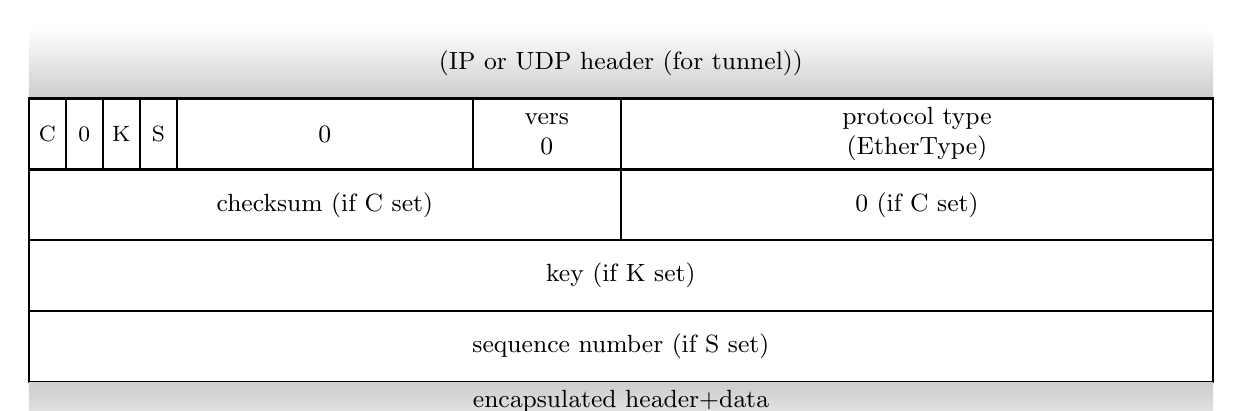
\begin{tikzpicture}
    \tikzset{
        box/.style={draw,thick},
        box unused/.style={draw,thick,pattern=north west lines},
        box label/.style={midway,font=\small,align=center},
        box label flags/.style={midway,font=\fontsize{8}{9}\selectfont,align=center},
        hi on/.style={},%alt=<#1>{ultra thick,fill=red!10}},
        explain box 1/.style={draw=red,line width=0.8mm,fill=white,anchor=center,at={(explain box loc 1)},align=center},
        explain box 2/.style={draw=red,line width=0.8mm,fill=white,anchor=center,at={(explain box loc 2)},align=center},
        explain box 3/.style={draw=red,line width=0.8mm,fill=white,anchor=center,at={(explain box loc 3)},align=center},
    }
    \begin{scope}[x=4.7mm,y=9mm]
        \coordinate (explain box loc 1) at (16, -3.1);
        \coordinate (explain box loc 2) at (16, -5.1);
        \coordinate (explain box loc 3) at (16, -1.1);
        \path[shading=axis,top color=white,bottom color=black!20] (0, 1) rectangle (32, 0)
            node[box label] {(IP or UDP header (for tunnel))};
        \path[box,hi on=2] (0, 0) rectangle ++(1, -1) node[box label flags] {C};
        \path[box,hi on=0] (1, 0) rectangle ++(1, -1) node[box label flags] {0};
        \path[box,hi on=2,hi on=3] (2, 0) rectangle ++(1, -1) node[box label flags] {K};
        \path[box,hi on=2] (3, 0) rectangle ++(1, -1) node[box label flags] {S};
        \path[box,hi on=0] (4, 0) rectangle (12, -1) node[box label] {0};
        \path[box,hi on=0] (12, 0) rectangle (16, -1) node[box label] {vers\\0};
        \path[box,hi on=0] (16, 0) rectangle (32, -1) node[box label] {protocol type \\ (EtherType)};
        \path[box,hi on=0] (0, -1) rectangle (16, -2) node[box label] {checksum (if C set)};
        \path[box,hi on=0] (16, -1) rectangle (32, -2) node[box label] {0 (if C set)};
        \path[box,hi on=0,hi on=3] (0, -2) rectangle (32, -3) node[box label] {key (if K set)};
        \path[box,hi on=0] (0, -3) rectangle (32, -4) node[box label] {sequence number (if S set)};
        \path[overlay,shading=axis,top color=black!20,bottom color=white] (0, -4) rectangle (32, -5)
            node[box label] {
                encapsulated header+data \\
                (probably IPv4 or IPv6)
            };
    \end{scope}
\end{tikzpicture}
\end{frame}

\begin{frame}{TCP-in-TCP problems}
    \begin{itemize}
    \item sometimes run IP tunnel over TCP
        \begin{itemize}
        \item example: picky firewall rules, or non-UDP-supporting NAT
        \end{itemize}
    \item outer TCP connection adds extra buffering
        \begin{itemize}
        \item more than UDP, because will usually buffer instead of dropping
        \end{itemize}
    \vspace{.5cm}
    \item $\rightarrow$ very high round-trip time if not careful
    \item can result in very poor TCP performance
    \end{itemize}
\end{frame}


\section{link-layer granularity}

\subsection{VLANs}

\begin{frame}{VLAN idea}
    \begin{itemize}
    \item multiple (`virtual') local networks over one network
    \item links/ports either shared or assigned to just one network
    \item most common implementation: Ethernet 801.1q:
    \vspace{.5cm}
    \item on shared links, frames tagged with their `VLAN ID'
        \begin{itemize}
        \item special case: untagged frames part of VLAN ID 0x0
        \end{itemize}
    \item tags added/removed when going to unshared links
        \begin{itemize}
        \item and broadcast frames filtered out if VLAN ID doesn't match
        \end{itemize}
    \end{itemize}
\end{frame}

\begin{frame}[fragile]{Ethernet encapsulation}
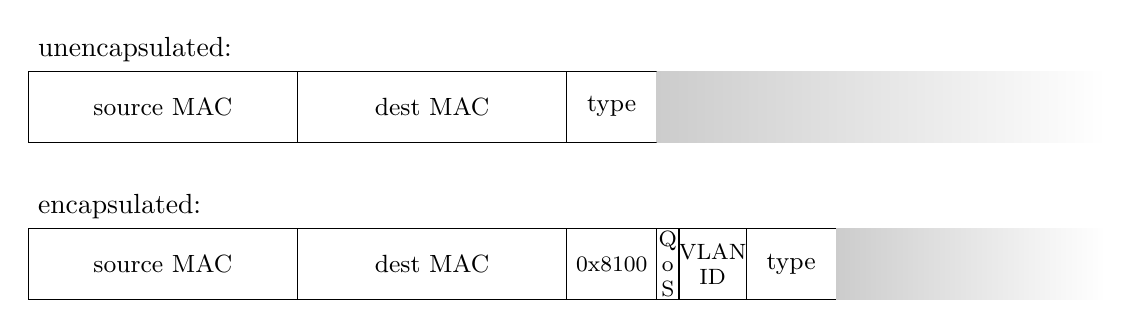
\begin{tikzpicture}
    \tikzset{
        box/.style={draw,thick},
        box unused/.style={draw,thick,pattern=north west lines},
        box label/.style={midway,font=\small,align=center},
        box label flags/.style={midway,font=\fontsize{8}{9}\selectfont,align=center},
        hi on/.style={alt=<#1>{ultra thick,fill=red!10}},
        explain box 1/.style={draw=red,line width=0.8mm,fill=white,anchor=center,at={(explain box loc 1)},align=center},
        explain box 2/.style={draw=red,line width=0.8mm,fill=white,anchor=center,at={(explain box loc 2)},align=center},
        explain box 3/.style={draw=red,line width=0.8mm,fill=white,anchor=center,at={(explain box loc 3)},align=center},
    }
    \begin{scope}[x=5.7mm,y=9mm]
        \node[anchor=south west] at (0, 0) {unencapsulated:};
        \coordinate (explain box loc 1) at (16, -6.1);
        \draw (0, 0) rectangle ++(6, -1) node[box label]{source MAC};
        \draw (6, 0) rectangle ++(6, -1) node[box label]{dest MAC};
        \draw (12, 0) rectangle ++(2, -1) node[box label]{type};
        \path[shading=axis,right color=white, left color=black!20] (14, 0) rectangle (24, -1);
    \end{scope}
    \begin{scope}[x=5.7mm,y=9mm,yshift=-2cm]
        \node[anchor=south west] at (0, 0) {encapsulated:};
        \draw (0, 0) rectangle ++(6, -1) node[box label]{source MAC};
        \draw (6, 0) rectangle ++(6, -1) node[box label]{dest MAC};
        \draw (12, 0) rectangle ++(2, -1) node[box label flags]{0x8100};
        \draw (14, 0) rectangle ++(.5, -1) node[box label flags]{Q\\o\\S};
        \draw (14.5, 0) rectangle ++(1.5, -1) node[box label flags]{VLAN\\ID};
        \draw (16, 0) rectangle ++(2, -1) node[box label]{type};
        \path[shading=axis,right color=white, left color=black!20] (18, 0) rectangle (24, -1);
    \end{scope}
\end{tikzpicture}
\begin{itemize}
    \item network IDs (`VLAN identifiers') configured by sysadmins
        \begin{itemize}
        \item special case: 0x0 = default (untagged), 0xFFF = reserved
        \end{itemize}
    \item encapsulation typically added/removed by switches
    \item usually increase in supported frame size to accomodate tag
\end{itemize}
\end{frame}

\begin{frame}
    \frametitle{configuring Ethernet encapsulation}
    \begin{itemize}
    \item adding/removing VLAN identifiers --- options:
    \vspace{.5cm}
    \item configure switch to automatically tag input on specific ports and untag output
        \begin{itemize}
        \item example: some ports are `phone network', some are `desktop network'
        \item typically: ports for hosts add/remove tags; for other switches don't
        \end{itemize}
    \item end-hosts handle tagging/untagging
        \begin{itemize}
        \item example: each virtual machine assigned its own tag
        \item example: multiple `interfaces', each with own tag + IP address + routing
        \end{itemize}
    \end{itemize}
\end{frame}




\subsection{MPLS}

\usetikzlibrary{arrows.meta,calc,matrix,patterns,shapes}
\providecommand{\computer}{%
    \includegraphics[width=1cm]{../common/Noun_project_216.pdf}
}
\providecommand{\switch}{%
    \includegraphics[width=0.9cm]{../common/fig-switch.pdf}
}
\providecommand{\bigswitch}{%
    \includegraphics[width=1.4cm]{../common/fig-switch.pdf}
}
\providecommand{\router}{%
    \includegraphics[width=0.9cm]{../common/fig-router.pdf}
}



\begin{frame}[fragile]{multiprotocol label switching (MPLS)}
    \begin{itemize}
    \item MPLS: combines encapsulation and routing tables
    \end{itemize}
\begin{tikzpicture}
\tikzset{
    box/.style={draw,thick},
    box unused/.style={draw,thick,pattern=north west lines},
    box label/.style={midway,font=\small,align=center},
    computer/.style={inner sep=0mm,outer sep=0mm,execute at begin node={\computer}},
    switch/.style={inner sep=0mm,outer sep=0mm,execute at begin node={\switch}},
    router/.style={inner sep=-.5mm,outer sep=0mm,execute at begin node={\router}},
    port/.style={pos=0.95,fill=white,circle,draw,inner sep=0mm},
    port beginning/.style={pos=0.05,fill=white,circle,draw,inner sep=0mm},
    box label flags/.style={midway,font=\fontsize{8}{9}\selectfont,align=center},
    hi on/.style={alt=<#1>{ultra thick,fill=red!10}},
    explain box 1/.style={draw=red,line width=0.8mm,fill=white,anchor=center,at={(explain box loc 1)},align=center},
    explain box 2/.style={draw=red,line width=0.8mm,fill=white,anchor=center,at={(explain box loc 2)},align=center},
    explain box 3/.style={draw=red,line width=0.8mm,fill=white,anchor=center,at={(explain box loc 3)},align=center},
    route table/.style={
        matrix of nodes,ampersand replacement=\&,
        column sep=-.3mm, row sep=-.3mm,
        nodes={align=center,font=\fontsize{9}{10}\selectfont\tt,text depth=1mm,text height=3mm,minimum height=0.4cm,inner sep=0mm,draw,line width=.3mm},
        column 1/.style={nodes={text width=.7cm}},
        column 2/.style={nodes={text width=0.7cm}},
        column 3/.style={nodes={text width=1.7cm,font=\fontsize{7}{8}\selectfont\tt}},
        column 4/.style={nodes={text width=1.5cm}},
        column 5/.style={nodes={text width=.5cm}},
        row 1/.style={nodes={draw=none,font=\fontsize{9}{10}\selectfont}},
    },
    route table no in no dest/.style={
        matrix of nodes,ampersand replacement=\&,
        column sep=-.3mm, row sep=-.3mm,
        nodes={align=center,font=\fontsize{9}{10}\selectfont\tt,text depth=1mm,text height=3mm,minimum height=0.4cm,inner sep=0mm,draw,line width=.3mm},
        column 1/.style={nodes={text width=0.7cm}},
        column 2/.style={nodes={text width=1.5cm}},
        column 3/.style={nodes={text width=.5cm}},
        row 1/.style={nodes={draw=none,font=\fontsize{9}{10}\selectfont}},
    },
    route table no dest no in/.style={route table no in no dest},
    connect/.style={draw,very thick},
    msg/.style={
        matrix of nodes,nodes={draw,violet,line width=.3mm,font=\fontsize{8}{9}\selectfont\tt,
            inner sep=0mm,inner xsep=.5mm,text height=3mm,text depth=.5mm},
        fill=white,
        column sep=-.3mm,inner sep=0mm
    },
    >=Latex,
    hi row/.style 2 args={
        alt=<#1>{
            row #2/.style={nodes={fill=red!15}}
        }
    },
}
\node[router] (in0) at (0, 6) {};
\draw[connect,->] (-1, 7) -- (in0.north west) node[port]{0};
%\draw[connect,->] (-1, 6) -- (in0.west) node[port]{1};
\matrix[route table,anchor=north,hi row={2}{2}] at (0, 5.5) {
in \& label \& dest \& op \& out \\
0\& --- \& 3fff:1::/32 \& push 4 \& 2 \\
0 \& --- \& 3fff:2::/32 \& push 7 \& 2 \\
2 \& 9 \& --- \& pop \& 0\\
\ldots \& \ldots \& \ldots \& \ldots \& \ldots \\
};
\node[router] (out0) at (10, 8) {};
\draw[connect,->] (out0.east) -- ++(.5, 0) node[right,font=\tiny\tt] {3fff:1::/32}
    node[port beginning] {1};
\draw[connect,->] (out0.north east) -- ++(.5, .5)
    node[port beginning] {2};
\node[router] (out1) at (5, 4) {};
\draw[connect,->] (out1.south) -- ++(0, -.5) node[right,font=\tiny\tt] {3fff:2::/32}
    node[port beginning] {1};
\node[router,alt=<5>{fill=red!10}] (mid1) at (5, 6) {};
\matrix[alt=<5>{draw=red,very thick},route table no in no dest,anchor=south,hi row={2-4}{2}] (mid1 table) at ([xshift=-1.5cm]mid1.north) {
label \& op \& out \\
24 \& swap 1 \& 21 \\
25 \& swap 2 \& 21 \\
27 \& swap 1 \& 22 \\
28 \& swap 9 \& 0 \\
\ldots \& \ldots \& \ldots \\
};
\matrix[route table,anchor=north,hi row={2}{4}] at ([yshift=-.3cm]out0.south) {
in \& label \& dest \& op \& out \\
1 \& --- \& 3fff:2::/32\& push 27 \& 0\\
1 \& --- \& default \& push 28 \& 0\\
0 \& 21 \& --- \& pop \& 21 \\
0 \& 22 \& --- \& pop \& 22 \\
\ldots \& \ldots \& \ldots \& \ldots \& \ldots \\
};
\foreach \x/\y/\xp/\yp in {in0/mid1/2/0,mid1/out0/1/0,mid1/out1/2/0} {
    \draw[connect,<->] (\x) -- (\y) node[port beginning] {\xp} node[port] {\yp};
}
\begin{visibleenv}<2-4>
    \matrix[msg,anchor=south] at ([yshift=.5cm]in0.north west) {
        dest=3fff:1::aa \& \ldots \\
    };
    \matrix[msg,anchor=west] at ([xshift=.5cm]in0.east) {
        |[alt={<3>{fill=red!15}}]| 24 \& dest=3fff:1::aa \& \ldots \\
    };
    \matrix[msg,anchor=west] at ([xshift=.5cm,yshift=1cm]mid1.east) {
        |[alt={<3>{fill=red!15}}]| 21 \& dest=3fff:1::aa \& \ldots \\
    };
\end{visibleenv}
\begin{visibleenv}<3>
\node[align=left,draw=red,very thick,fill=white,anchor=west] at (mid1 table.east) {
    `swap' operation to translate \\
    between different label meanings \\
    ~ \\
    allows piecemail configuration
};
\end{visibleenv}
\begin{visibleenv}<5>
\node[align=left,draw=red,very thick,fill=white,anchor=west] at (mid1 table.east) {
    routers in `middle' of network \\
    have \textit{very simple} routing decisions \\
    no prefix matching
};
\end{visibleenv}
\end{tikzpicture}
\end{frame}

\begin{frame}{Label Distribution Protocol}
    \begin{itemize}
    \item share with neighbors list of:
        \begin{itemize}
        \item (ultimate destination, desired label)
        \end{itemize}
    \item use entries to
        \begin{itemize}
        \item allocate new local labels
        \item setup appropriate \texttt{swap} entries
        \item send other neighbors update about new labels
        \end{itemize}
    \vspace{.5cm}
    \item if using normal routing protocol to decide which neighbors routes to accept,
    just a funny way to implement routing tables
    \end{itemize}
\end{frame}

\begin{frame}[fragile]{MPLS tunnel}
\begin{tikzpicture}
\tikzset{
    box/.style={draw,thick},
    box unused/.style={draw,thick,pattern=north west lines},
    box label/.style={midway,font=\small,align=center},
    computer/.style={inner sep=0mm,outer sep=0mm,execute at begin node={\computer}},
    switch/.style={inner sep=0mm,outer sep=0mm,execute at begin node={\switch}},
    router/.style={inner sep=-.5mm,outer sep=0mm,execute at begin node={\router}},
    port/.style={pos=0.95,fill=white,circle,draw,inner sep=0mm},
    port beginning/.style={pos=0.05,fill=white,circle,draw,inner sep=0mm},
    box label flags/.style={midway,font=\fontsize{8}{9}\selectfont,align=center},
    hi on/.style={alt=<#1>{ultra thick,fill=red!10}},
    explain box 1/.style={draw=red,line width=0.8mm,fill=white,anchor=center,at={(explain box loc 1)},align=center},
    explain box 2/.style={draw=red,line width=0.8mm,fill=white,anchor=center,at={(explain box loc 2)},align=center},
    explain box 3/.style={draw=red,line width=0.8mm,fill=white,anchor=center,at={(explain box loc 3)},align=center},
    route table/.style={
        matrix of nodes,ampersand replacement=\&,
        column sep=-.3mm, row sep=-.3mm,
        nodes={align=center,font=\fontsize{9}{10}\selectfont\tt,text depth=1mm,text height=3mm,minimum height=0.4cm,inner sep=0mm,draw,line width=.3mm},
        column 1/.style={nodes={text width=.7cm}},
        column 2/.style={nodes={text width=0.7cm}},
        column 3/.style={nodes={text width=1.7cm,font=\fontsize{7}{8}\selectfont\tt}},
        column 4/.style={nodes={text width=1.5cm}},
        column 5/.style={nodes={text width=.5cm}},
        row 1/.style={nodes={draw=none,font=\fontsize{9}{10}\selectfont}},
    },
    route table no in no dest/.style={
        matrix of nodes,ampersand replacement=\&,
        column sep=-.3mm, row sep=-.3mm,
        nodes={align=center,font=\fontsize{9}{10}\selectfont\tt,text depth=1mm,text height=3mm,minimum height=0.4cm,inner sep=0mm,draw,line width=.3mm},
        column 1/.style={nodes={text width=0.7cm}},
        column 2/.style={nodes={text width=1.5cm}},
        column 3/.style={nodes={text width=.5cm}},
        row 1/.style={nodes={draw=none,font=\fontsize{9}{10}\selectfont}},
    },
    route table no dest/.style={
        matrix of nodes,ampersand replacement=\&,
        column sep=-.3mm, row sep=-.3mm,
        nodes={align=center,font=\fontsize{9}{10}\selectfont\tt,text depth=1mm,text height=3mm,minimum height=0.4cm,inner sep=0mm,draw,line width=.3mm},
        column 1/.style={nodes={text width=0.7cm}},
        column 2/.style={nodes={text width=0.7cm}},
        column 3/.style={nodes={text width=1.5cm}},
        column 4/.style={nodes={text width=.5cm}},
        row 1/.style={nodes={draw=none,font=\fontsize{9}{10}\selectfont}},
    },
    route table no dest no in/.style={route table no in no dest},
    connect/.style={draw,very thick},
    msg/.style={
        matrix of nodes,nodes={draw,violet,line width=.3mm,font=\fontsize{8}{9}\selectfont\tt,
            inner sep=0mm,inner xsep=.5mm,text height=3mm,text depth=.5mm},
        fill=white,
        column sep=-.3mm,inner sep=0mm},
    >=Latex,
    hi row/.style 2 args={
        alt=<#1>{
            row #2/.style={nodes={fill=red!15}}
        }
    },
}

\node at (6, 9) {logical view --- `virtual wire'};
\node (log A) at (-2, 8.5) {A};
\node (log B) at (13, 8.5) {B};
\draw[connect,<->] (log A) -- (log B);

\draw[overlay, ultra thick] (-3.5, 7.8) -- (14, 7.8);

\node[anchor=north] at (6, 7.8) {actual network};

\node[router] (in0) at (0, 6) {};
\draw[connect,<->] (-1.5, 6) -- (in0.west) node[port]{0}
    node[pos=0,left] {A};
\matrix[route table no dest,anchor=north] at (0, 5.5) {
in \& label  \& op \& out \\
0 \& ---  \& push 32 \& 1 \\
--- \& 1 \& pop \& 0 \\
\ldots \& \ldots \& \ldots \& \ldots \\
};
\node[router] (mid1) at (4, 6) {};
\matrix[route table no dest no in,anchor=north] at (4, 4) {
label  \& op \& out \\
32 \& swap 37 \& 4 \\
26 \& swap 21 \& 0 \\
\ldots \& \ldots \& \ldots \\
};
\node[router] (mid2) at (8, 6) {};
\matrix[route table no dest no in,anchor=north] at (8, 5.5) {
label  \& op \& out \\
37 \& swap 20 \& 6 \\
39 \& swap 32 \& 3 \\
\ldots \& \ldots \& \ldots \\
};
\node[router] (out0) at (11, 6) {};
\matrix[route table no dest,anchor=north] at (11, 4) {
in \& label  \& op \& out \\
0 \& --- \& push 37 \& 1 \\
--- \& 0 \& swap 29 \& 6 \\
\ldots \& \ldots \& \ldots \& \ldots \\
};
\draw[connect,->](out0.east) -- ++(1, 0) node[port beginning]{0}
    node[pos=1,right] {B};

\foreach \x/\y in {mid1/30,mid1/60,mid1/270,mid2/45,mid2/90,mid2/210,mid2/290,
                   in0/90,in0/270,out0/60,out0/280} {
    \draw[connect,<-] (\x.\y) -- ++(\y:.5cm);
};
\foreach \x/\y/\xp/\yp in {in0/mid1/1/0,mid1/mid2/4/3,mid2/out0/6/1} {
    \draw[connect,<->] (\x) -- (\y) node[port beginning] {\xp} node[port] {\yp};
}
\end{tikzpicture}
\end{frame}

\begin{frame}{MPLS tunnels for traffic engineering}
    \begin{itemize}
    \item if multiple paths from A to B often want to:
        \begin{itemize}
        \item balance between them to use available bandwidth
        \item prioritize important traffic on `better' path
        \item \ldots
        \end{itemize}
    \item plain OSPF can't really do any of this unless equal cost
    \vspace{.5cm}
    \item MPLS gives mechanism to do this kind of balancing:
        \begin{itemize}
        \item setup labels along desired paths
        \item choosing new path (or failover) = changing `swap X' to `swap Y'
        \item can configure backup paths in advance and turn them on later
        \end{itemize}
    \end{itemize}
\end{frame}

\begin{frame}[fragile]{rapid failover}
\begin{tikzpicture}
\tikzset{
    box/.style={draw,thick},
    box unused/.style={draw,thick,pattern=north west lines},
    box label/.style={midway,font=\small,align=center},
    computer/.style={inner sep=0mm,outer sep=0mm,execute at begin node={\computer}},
    switch/.style={inner sep=0mm,outer sep=0mm,execute at begin node={\switch}},
    router/.style={inner sep=-.5mm,outer sep=0mm,execute at begin node={\router}},
    port/.style={pos=0.95,fill=white,circle,draw,inner sep=0mm},
    port beginning/.style={pos=0.05,fill=white,circle,draw,inner sep=0mm},
    box label flags/.style={midway,font=\fontsize{8}{9}\selectfont,align=center},
    hi on/.style={alt=<#1>{ultra thick,fill=red!10}},
    explain box 1/.style={draw=red,line width=0.8mm,fill=white,anchor=center,at={(explain box loc 1)},align=center},
    explain box 2/.style={draw=red,line width=0.8mm,fill=white,anchor=center,at={(explain box loc 2)},align=center},
    explain box 3/.style={draw=red,line width=0.8mm,fill=white,anchor=center,at={(explain box loc 3)},align=center},
    route table/.style={
        matrix of nodes,ampersand replacement=\&,
        column sep=-.3mm, row sep=-.3mm,
        nodes={align=center,font=\fontsize{9}{10}\selectfont\tt,text depth=1mm,text height=3mm,minimum height=0.4cm,inner sep=0mm,draw,line width=.3mm},
        column 1/.style={nodes={text width=.7cm}},
        column 2/.style={nodes={text width=0.7cm}},
        column 3/.style={nodes={text width=1.7cm,font=\fontsize{7}{8}\selectfont\tt}},
        column 4/.style={nodes={text width=1.5cm}},
        column 5/.style={nodes={text width=.5cm}},
        row 1/.style={nodes={draw=none,font=\fontsize{9}{10}\selectfont}},
    },
    route table no in no dest/.style={
        matrix of nodes,ampersand replacement=\&,
        column sep=-.3mm, row sep=-.3mm,
        nodes={align=center,font=\fontsize{9}{10}\selectfont\tt,text depth=1mm,text height=3mm,minimum height=0.4cm,inner sep=0mm,draw,line width=.3mm},
        column 1/.style={nodes={text width=0.7cm}},
        column 2/.style={nodes={text width=1.5cm}},
        column 3/.style={nodes={text width=.5cm}},
        row 1/.style={nodes={draw=none,font=\fontsize{9}{10}\selectfont}},
    },
    route table no dest/.style={
        matrix of nodes,ampersand replacement=\&,
        column sep=-.3mm, row sep=-.3mm,
        nodes={align=center,font=\fontsize{9}{10}\selectfont\tt,text depth=1mm,text height=3mm,minimum height=0.4cm,inner sep=0mm,draw,line width=.3mm},
        column 1/.style={nodes={text width=0.7cm}},
        column 2/.style={nodes={text width=0.7cm}},
        column 3/.style={nodes={text width=1.5cm}},
        column 4/.style={nodes={text width=.5cm}},
        row 1/.style={nodes={draw=none,font=\fontsize{9}{10}\selectfont}},
    },
    route table no dest no in/.style={route table no in no dest},
    connect/.style={draw,very thick},
    msg/.style={
        matrix of nodes,nodes={draw,violet,line width=.3mm,font=\fontsize{8}{9}\selectfont\tt,
            inner sep=0mm,inner xsep=.5mm,text height=3mm,text depth=.5mm},
        fill=white,
        column sep=-.3mm,inner sep=0mm},
    >=Latex,
    hi row/.style 2 args={
        alt=<#1>{
            row #2/.style={nodes={fill=red!15}}
        }
    },
}

\draw[connect,<->] (-1.5, 6) -- (in0.west) node[port]{0};
\node[router] (in0) at (0, 6) {};
\matrix[route table no dest no  in,anchor=north] at (0, 5.5) {
label  \& op \& out \\
21 \& swap 25 \& 1 \\
(backup) 21 \& swap 27 \& 2 \\
27 \& swap 30 \& 0 \\
 \ldots \& \ldots \& \ldots \\
};
\node[router] (mid1) at (12, 6) {};
\matrix[route table no dest no in,anchor=north] at (12, 5.5) {
label  \& op \& out \\
25 \& swap 27 \& 3 \\ 
 \ldots \& \ldots \& \ldots \\
};
\node[router] (out0) at (6, 4) {};
\matrix[route table no dest no in,anchor=north] at (6, 3.5) {
label  \& op \& out \\
27 \& swap 24 \& 3 \\
28 \& swap 25 \& 1 \\
\ldots \& \ldots \& \ldots \\
};
\draw[connect,<->] (-13.5, 6) -- (out0.east) node[port]{1};
\foreach \x/\y/\xp/\yp in {in0/out0/1/1,in0/mid1/2/1,mid1/out0/3/2} {
    \draw[connect,<->] (\x) -- (\y) node[port beginning] {\xp} node[port] {\yp};
}
\end{tikzpicture}
\end{frame}

\begin{frame}{RSVP-TE}
    \begin{itemize}
    \item RSVP-TE (RFC 3209): protocol for setting up MPLS tunnels
    \item idea: routers figure out labels, etc.
    \item end-user can (optionally) specify\ldots
    \vspace{.5cm}
    \item that tunnel go through specific routers
    \item also setting up `fast reroute' backup paths
    \item bandwidth reservation 
        \begin{itemize}
        \item routers give you error if bandwidth not gaurenteed
        \end{itemize}
    \end{itemize}
\end{frame}

\begin{frame}{nested labels}
    \begin{itemize}
    \item label \textit{stack} allows \ldots
    \item nested tunnels
    \item marking different types of packet
    \item \ldots
    \end{itemize}
\end{frame}

\begin{frame}{protocol-independence}
    \begin{itemize}
    \item only first/last routers care about actual protocol
    \item easily allows for\ldots
    \vspace{.5cm}
    \item mix of Ethernet and IP tunnels
    \item using routers that don't support IP (e.g. ATM)
    \item \ldots
    \end{itemize}
\end{frame}

\begin{frame}[fragile]{actual label format}
\begin{Verbatim}[fontsize=\small]
 0                   1                   2                   3
 0 1 2 3 4 5 6 7 8 9 0 1 2 3 4 5 6 7 8 9 0 1 2 3 4 5 6 7 8 9 0 1
+-+-+-+-+-+-+-+-+-+-+-+-+-+-+-+-+-+-+-+-+-+-+-+-+-+-+-+-+-+-+-+-+ Label
|                Label                  | Exp |S|       TTL     | Stack
+-+-+-+-+-+-+-+-+-+-+-+-+-+-+-+-+-+-+-+-+-+-+-+-+-+-+-+-+-+-+-+-+ Entry

                    Label:  Label Value, 20 bits
                    Exp:    Experimental Use, 3 bits
                    S:      Bottom of Stack, 1 bit
                    TTL:    Time to Live, 8 bits
\end{Verbatim}
\begin{itemize}
\item TTL here is different than we've seen:
\item only processed when label popped
\item typically (re)set to mirror IP TTL if MPLS run over IP
\end{itemize}
\end{frame}





\section{backup slides}
\begin{frame}\frametitle{backup slides}
\end{frame}

\begin{frame}[label=pktFilterExamples]{why packet filtering}
    \begin{itemize}
    \item some reasons to \textit{filter} packets:
    \vspace{.5cm}
    \item remove (malicious?) packets with false source addresses
    \item disallow external access to servers not on allowlist
    \item block traffic from known malicious sources
    \item only permit services on allowlist out of private network
    \end{itemize}
\end{frame}


\section{firewall: placement, state}
\begin{frame}{packet filters = firewalls}
    \begin{itemize}
    \item typical name for packet filter: ``firewall''
    \item especially filtering focused on security
    \end{itemize}
\end{frame}

\begin{frame}<1>[label=ffDesign]{firewall design decisions}
    \begin{itemize}
    \item where to filter?
        \begin{itemize}
        \item typically: \myemph<2>{at ``edges'' of network}
        \item in router, or separate box
        \item can also do elsewhere
        \end{itemize}
    \item how much to track when filtering?
        \begin{itemize}
        \item ``stateless'' or ``stateful''
        \end{itemize}
    \end{itemize}
\end{frame}

\againframe<2>{ffDesign}
\begin{frame}{the corporate firewall}
\includegraphics[width=0.9\textwidth]{sysapp-fig214}
\end{frame}



\subsection{zones of trust idea}
\begin{frame}{zones of trust}
    \begin{itemize}
    \item most common kind of firewall policy, three zones:
    \item internal network
        \begin{itemize}
        \item can send most things
        \item can't receive unsolicited traffic from external network
        \item where typical laptops/desktops live
        \end{itemize}
    \item DMZ (`demilitrized zone')
        \begin{itemize}
        \item not `protected' from external networks
        \item access to internal network similar to being within it
        \item where externally accessible services live
        \end{itemize}
    \item external network
        \begin{itemize}
        \item can only unsolicited to DMZ
        \item where the rest of the Internet lives
        \end{itemize}
    \end{itemize}
\end{frame}



\end{document}
